\documentclass{article}
\usepackage[utf8]{inputenc}

\title{Lecture 7: resampeling methods }
\author{wbg231 }
\date{November 2022}
\usepackage{tikz,graphicx,amsmath,amsfonts,amscd,amssymb,bm,cite,epsfig,epsf,url}
\begin{document}

\maketitle

\section{introduction}
\subsection{limitations to parametric tests}
\begin{itemize}
%\item 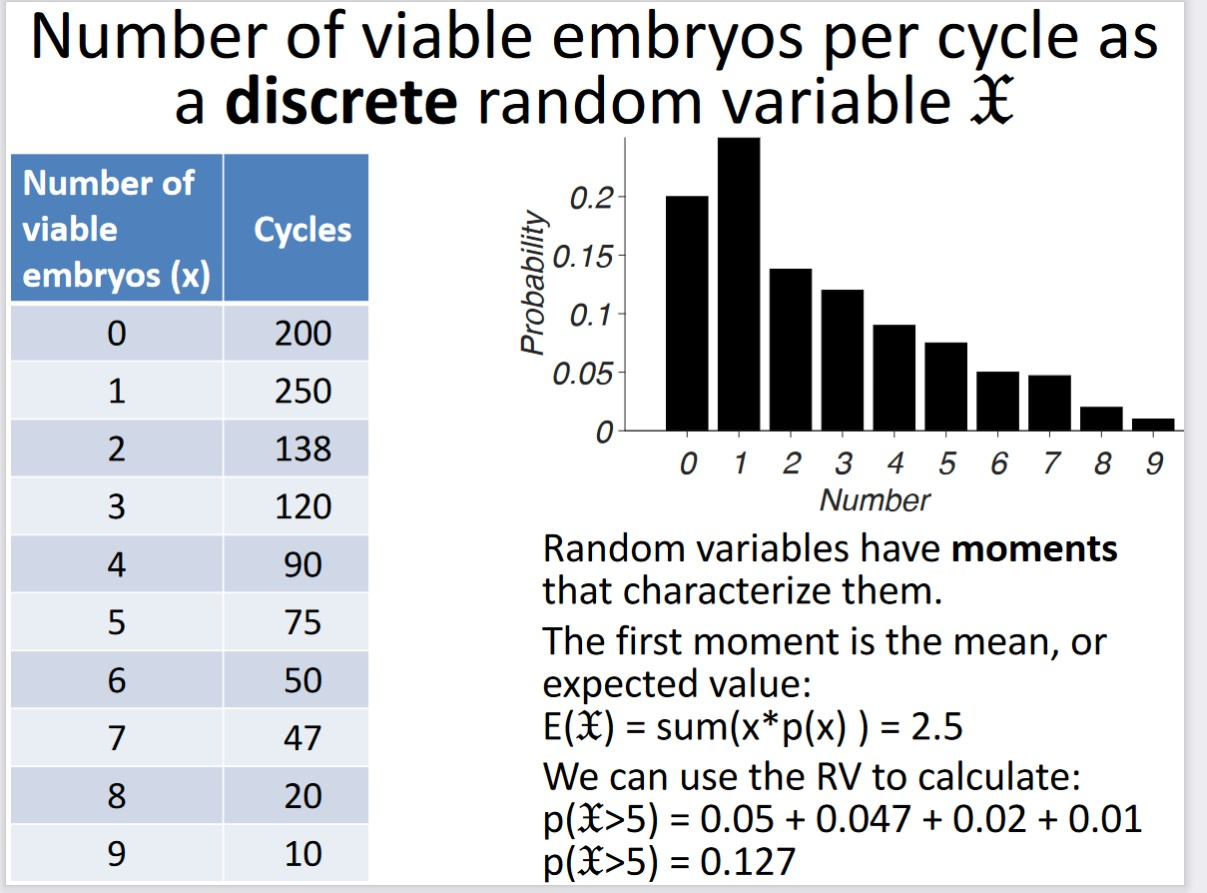
\includegraphics[width=7.5cm]{Final_Review/Lecture_2/lecture_1example.jpg}
\item there are limitations to classical parametric tests 
\item for instance we have to make a lot of assumptions, and if those assumptions are violated the tests work poorly
\item there are also some use cases that are very complex and it is unclear which to use
\item the distribution of the test statistic under the null is an approximation and assumes that n is near infinity. which may not hold
\section{permutation test}
\item $\{a,b,c\}$ a permutation is an order set so that set up there has 6 permutations 
\subsection{example}
\item there are two types of galaxies spiral and elliptical 
\item question: do these types of galaxies differ in terms of how many pulsars they have? 
\item suppose we count the number of pulsars in 5 galaxies of each type 
\item our null is that  the difference in the number of pulsars is not different 
\item we know nothing about astronomy so we are not sure what test to use
\item so what can we do? we can make our own test ie the permutation test
\item the permeation test makes almost no assumptions
\subsection{INTRODUCING THE permutation test}
\item if we have a problem where we do now know what to expect in terms of the test stat (which one to use and how it distributes under the null this is a good use case 
\item if our assumptions in a classical test are violated our test is biased.
\item so instead of making assumptions to solve this problem. We just use the actual data we have to determine the distribution of the test stat under the null hypothesis and the null distribution 
\item this is kind of similar to ml in that we are completely focused on the data. 
\item if the data is assumptions are met the traditional tests will likely be more powerful
\subsection{defining a test stat }
\item in principle the value of a test stat should be large when the null is false and small then the null is true 
\item but we don't need to follow this necessarily 
\item suppose we just same our test stat is $sum(x_1)-sum(x_2)$ that is the difference in the sum of two pulsars
\item we are making many  assumptions 
\begin{itemize}
    \item first that they are of the same length, because a list of a longer length will likely be larger
    \item does sign matter if so we should square
\end{itemize}
\item we could come up with many test stats that have different properties, and may have different results.
\subsection{ test stat choice is not trivial }
\item 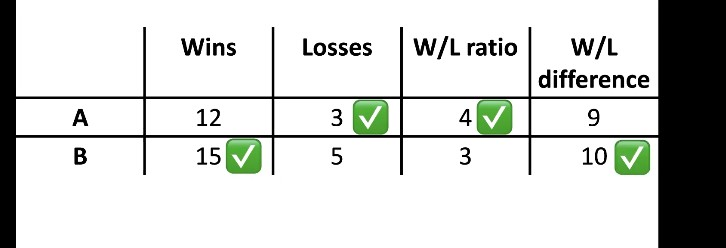
\includegraphics[width=7.5cm]{Final_Review/lecture_7/test_stat_exmaple.jpg}
\item two people are playing tennis. 
\item we use wins as a test stat b is better 
\item if we count losses as a test stat a is better 
\item if we use the win loss ratio a is better 
\item etc 
\item so who is the better player, it depends on the test stat we chose. 
\subsection{null hypothesis oif test stat}
\item suppose we have defined a test statistic our next goal is to determine, the distribution of that test statistic under the null hypothesis
\item the logic is we pretend we lost the labels for each sample (ie an element from either could be drawn)
\item then we form synthetic groups of the same size as the original data set from the data at random without replacement (so if we have two samples of size 5, we draw 5 random samples with out replacement from either group n times) 
\item then calculate the test stat of one such randomly create set of groups
\item to determine the null distribution of this test stat we repeat this many times 
\itme this is called permutation test because we are drawing with out replacement so we are shuffling different subsets.
\item drawing with out replacement maps all elements form the data set to the re samples set this is one to one and onto. in other words each elements in b comes form a single element in a. this is a bijective function this is nice to work with 
\itme drawing with replacement, is not bijective so it is just harder to work with mathematically. 
\item so when we empirically calculate our test stat, we need to take the test stat of many permutation of our samples to understand the null distribution of each test stat. 
\item doing this re sampling many times allows us to do this many times 
\item then we want to count how many of the simulated test stats are higher than our empirical test statistic, we call that our exact p-value 
\item how would we make this two tailed? we would take the absolute value of the test statistic and see if that is less than our alpha!
\item our null distribution will be lumpy if our original samples are small. if we had larger samples we would likely have a more smooth distribution

\subsection{permutation test summary}
\item use case if we are not sure what test to use, we don't want to make the assumptions of the standard tests, our are n is small
\begin{enumerate}
    \item design a test statistic that captures something of interest about the empirical sample. know what the assumptions of this test static are 
    \item compute the empirical test stat 
    \item randomly shuffle our empirical samples many times by drawing with out replacement 
    \item cut the shuffled data into groups that have the same size as the original group but otherwise at random 
    \item compute the shuffled test statistic for each of these synthetic groups
    \item the distribution of these shuffled test stats is our null distribution
    \item determine the area under the null more extreme than your empirically test statistic call this the exact p value 
    \item determine if this exact p value is significant 
    
    \end{enumerate}
    \section{bootsraping- sampling with replacement}
    \subsection{example}
    \item aspirin is linked to lower heart attack rates. this might not be causal, so we run a randomized experiment to test this, but then after getting initial results we can no longer do the study for ethical reasons 
    \item but we do not know how likely our test statistic is due to chance. 
    \item replication is out of the question 
    \subsection{this is a tall order}
    \item want to get form 1 sample both the empirical sample mean and how the sample mean distributes
\subsection{bootstrapping procedure}
\item this allows you to calculate form one sample how the sample mean would distribute 
\item we re sample with replacement form our empirical sample 
\item we do this N a very large time 
\item then we take the mean of each of these samples samples 
\item sort these sample mean sin order of magnitude and this will be our null distribution 
\item then we determine the boundary that contains a large proportion of the tyhcanic mean (usually 95\% or 99\%
\item then we compare this with our figure of interest (in this case it would be the idea that the ratio between the mean of the control and treatment groups are 1) 
\item if our figure of interest is outside of the interval we reject the null
\subsection{example}
\item 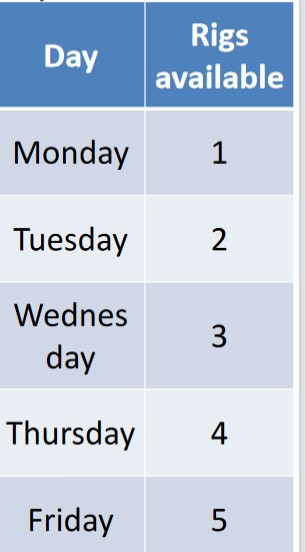
\includegraphics[width=7.5cm]{Final_Review/lecture_7/rig_chart.jpg}
\item gathering data for an experiment
\item you are only able to work one day a week chosen at random each week. each day has a different number of rigs available you need to work with 180 rigs within a year to complete your task
\item after 1 week the distribution is uniform 
\item after may weeks it starts to emerge to a uniform dist
\item we determine if we will make this
\subsection{clt and bootstrapping}
\item the boostrap applies the clt to the sample
\item the logic of the bootstrap is that instead of sampling form reality we sample form sample (with replacement) 
\item there are unknown population mean and std $\mu, \sigma$
\item we can draw a sample is hopefully Representative of the population call it $x_{empc}$ 
\item but it was really hard to get that sample, so instead of sampling from reality, we sample form the sample
\item we from sub samples with replacement $x_1....x_n$ which each have a sample mean. 
\item three things to notice
\begin{enumerate}
    \item we use the sample as a stand in for reality
    \item doing this we get different outcomes by sampling 
    \item the distribution of the sub samples, represent the conditions in the original sample we view this as our null hypothesis
\end{enumerate}
\item
\subsection{use cases}
\item we have limited data- it is very hard to get data, for instance there are only a few rare monkey skulls (this should only be done when there is no other option)
\item when we are unclear how the underlying distribution distributes or is unknown 
\item if we are estimating something that is really rare (this works well with a really large sample size) 

\subsection{bootstrap drawbacks and assumptions}
\item this works if and only if the sample is truly representative of the population
\item so this fails if there is sampling error or sampling bias
\item if there is sample bias, for instance all the earliest paintings  we have found are in caves, but it could be the case that there were others that have just not survived. so the cave paintings could not be Representative of the population
\item a small sample will necessarily under or over estimate the probability of rare events
\item this also does not work with ergotic data, because a sample is unlikely to capture very extreme values that are not the rare. 
\item we live in Portland, there has not been an earthquake in 300 years, our boots rapping model would say don't worry about it, but in 1700 there was a massive earthquake. so a large earthquake coming for Portland is real 
\item so just because it did not happen in your sample does not mean it can not happen 
\item large samples handle sampling error but not sampling bias 
\subsection{where the bootstrap name comes from}
\item pulling yourself up by your boot straps should work in reality but does not 
\item boots rapping is something that should not work, but does
\item boot strapping is a stochastic approximation of the jack knife. 
\item the jack knife is a deterministic leave one out method 
\subsection{jack knife }
\item we have a dataset of n individuals 
\item  we re sample from this data set some large number of times systematically leaving one data point out each time (so we have n-1 individuals in each of our subset samples) 
\item say our oringal data is $X=\{x_1..x_n\}$
\item we can calculate our sample mean as $\bar{x}=\frac{1}{n}\Sigma_{i=1}^{n}x_i$
\item suppose for each sub sample $x_j$ we leave out data point j from its calculation then our sub sample $x_j$ has means (note that the j matches the index) $\Bar{x_j}=\frac{1}{n-1}(\Sigma_{i=1}^{j-1}x_i+\Sigma_{i=j+1}^{n}x_i)$
\item so doing this we can calculate n subsets $x_i$ of size (n-1) which each have a mean $\Bar{x_i}$ 
\item so from this we can get variance estimate of the mean $\sigma_{x}=\Sigma_{i=1}^{n}\frac{\Bar{x_i}-\Bar{x}}{n(n-1)}$
\item this is a really good approximation of the true variance of the random viable 
\item the issue with this is the time complexity is bad, so in practice we use the bootstrap which is a stochastic approximation 
\subsection{back to Bootstrapping}
\item bootstrapping yields a confidence interval, and if our empirical mean is within 95\% of that we fail to reject the null
\item 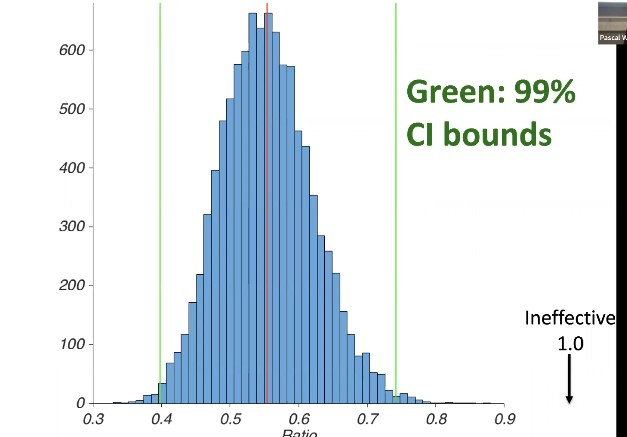
\includegraphics[width=7.5cm]{Final_Review/lecture_7/boostrapping_bounds .jpg}
 \item so in our example we end up with that boot strapping bounds 
\section{resampleing review}
\item permutation test: sampling with out replacement often to replace a significance test and get an exact p value for hypothesis testing 
\item bootstrapping:sampling with replacement often to compute the confidence interval of an empirical sample mean to access its stability. 
\item both of these work Best for large representative empirical samples
\item we need a high quality sample to ensure this works well
    


\end{itemize}
\end{document}
